% Chapter Template

\chapter{Some Examples} % Main chapter title

\label{Chapter3} % Change X to a consecutive number; for referencing this chapter elsewhere, use \ref{Chapter3}

\begin{sloppypar}
%----------------------------------------------------------------------------------------
% \addchaptertocentry{ABSTRACT}
% \begin{center}
%     {\centering\large\bfseries ABSTRACT}
% \end{center}
This chapter provides a number of examples for learning how to use latex for different needs. The examples are taken from various free templates present on the overleaf.com websites.

% \newpage

%----------------------------------------------------------------------------------------
%	SECTION 1
%----------------------------------------------------------------------------------------

\section{Main Section 1}

Lorem ipsum dolor sit amet, consectetur adipiscing elit. Aliquam ultricies lacinia euismod. Nam tempus risus in dolor rhoncus in interdum enim tincidunt \parencite{Reference2}. Donec vel nunc neque. In condimentum ullamcorper quam non consequat. Fusce sagittis tempor feugiat. Fusce magna erat, molestie eu convallis ut, tempus sed arcu. Quisque molestie, ante a tincidunt ullamcorper, sapien enim dignissim lacus, in semper nibh erat lobortis purus. Integer dapibus ligula ac risus convallis pellentesque.

%-----------------------------------
%	SUBSECTION 1
%-----------------------------------
\subsection{Subsection 1}

Nunc posuere quam at lectus tristique eu ultrices augue venenatis. Vestibulum ante ipsum primis in faucibus orci luctus et ultrices posuere cubilia Curae; Aliquam erat volutpat. Vivamus sodales tortor eget quam adipiscing in vulputate ante ullamcorper. Sed eros ante, lacinia et sollicitudin et, aliquam sit amet augue. In hac habitasse platea dictumst.

%-----------------------------------
%	SUBSECTION 2
%-----------------------------------

\subsection{Subsection 2}
Morbi rutrum odio eget arcu adipiscing sodales. Aenean et purus a est pulvinar pellentesque. Cras in elit neque, quis varius elit. Phasellus fringilla, nibh eu tempus venenatis, dolor elit posuere quam, quis adipiscing urna leo nec orci. Sed nec nulla auctor odio aliquet consequat. Ut nec nulla in ante ullamcorper aliquam at sed dolor. Phasellus fermentum magna in augue gravida cursus. Cras sed pretium lorem. Pellentesque eget ornare odio. Proin accumsan, massa viverra cursus pharetra, ipsum nisi lobortis velit, a malesuada dolor lorem eu neque.

%----------------------------------------------------------------------------------------
%	SECTION 2
%----------------------------------------------------------------------------------------

\section{Main Section 2}

Sed ullamcorper quam eu nisl interdum at interdum enim egestas. Aliquam placerat justo sed lectus lobortis ut porta nisl porttitor. Vestibulum mi dolor, lacinia molestie gravida at, tempus vitae ligula. Donec eget quam sapien, in viverra eros. Donec pellentesque justo a massa fringilla non vestibulum metus vestibulum. Vestibulum in orci quis felis tempor lacinia. Vivamus ornare ultrices facilisis. Ut hendrerit volutpat vulputate. Morbi condimentum venenatis augue, id porta ipsum vulputate in. Curabitur luctus tempus justo. Vestibulum risus lectus, adipiscing nec condimentum quis, condimentum nec nisl. Aliquam dictum sagittis velit sed iaculis. Morbi tristique augue sit amet nulla pulvinar id facilisis ligula mollis. Nam elit libero, tincidunt ut aliquam at, molestie in quam. Aenean rhoncus vehicula hendrerit.

\section{Mathematical Expressions}\label{maths}


%----------------------------------------------------------------------------------------
%	PROBLEM 1
%----------------------------------------------------------------------------------------

\subsection{Exercise 1}
% \lipsum[2] % Dummy text
(1) Given the distribution $\frac{1}{3\sqrt{2\pi}}e^{-\frac{1}{2}(\frac{x}{3})2}$ what is the probability that $x>1$?\par
Solution: 
\begin{align}
    \nonumber
    P(x>1)  &= \int_1^{\infty}\frac{1}{3\sqrt{2\pi}}xe^{-\frac{1}{2}(\frac{x}{3})^2}dx\\
    \nonumber
    &=\frac{1}{3\sqrt{2\pi}}\int_1^{\infty}\frac{1}{2}e^{-\frac{1}{18}x^2}dx^2~~~~~~~~~~~~~~~~~~(y\doteq \frac{1}{18}x^2)\\
    \nonumber
    &=\frac{3}{\sqrt{2\pi}}\int_{\frac{1}{18}}^{\infty}-e^{-y}dy\\
    \nonumber
    &=\frac{3}{\sqrt{2\pi}}e^{-\frac{1}{18}}
\end{align}

(2) Compare the Markov and Chebyshev bounds for the following probability distributions:\par

\begin{equation}
    \text{a})~~p(x)=\left\{
    \begin{array}{rl}
        1, & x=1\\
        0, & \text{otherwise}
    \end{array}\right.
\end{equation}
\begin{equation}
    \text{b})~~p(x)=\left\{
    \begin{array}{rl}
        \frac{1}{2}, & 0\leq x\leq 2\\
        0, & \text{otherwise}
    \end{array}\right.
\end{equation}

Solution:\\
For a), $E(x)=1$, $Var(x)=0$. So Markov inequality for a) is $Prob(x\geq a)\leq \frac{1}{a}$, while Chebyshev inequality for a) vanishes to $Prob(|x-1|>0)=0$.\par
For b), $E(x)=\int_0^2 \frac{1}{2}xdx=1$, $Var(x)=\int_0^2 \frac{1}{2}(x-1)^2dx=\frac{1}{3}$. So Markov inequality for b) is $Prob(x\geq a)\leq \frac{1}{a}$ (which is the same as in problem a)), while Chebyshev inequality for b) is $Prob(|x-1|>\sqrt{\frac{1}{3}}a)\leq \frac{1}{a^2}$.\par


(3) Let $s$ be the sum of $n$ independent ransom variables $x_1,x_2,\cdots,x_n$ where for each $i$,\par
\begin{equation}
    x_i=\left\{
    \begin{array}{rl}
        0, & \text{Prob is }p\\
        1, & \text{Prob is }1-p
    \end{array}\right.
\end{equation}

How large must $\delta$ be if we wish to have Prob($s>(1+\delta)n)<\epsilon$\par

Solution:\par
$E(x_i)=1-p,~Var(x)=(1-(1-p))^2(1-p)+(0-(1-p))^2p=p^2(1-p)+(1-p)^2p=p^2-p^3+p-2p^2+p^3=p-p^2$.\\ 
So $Prob(x\geq a)\leq \frac{1-p}{a}$ for each $i$. So $E(s)=n(1-p)$, $Var(s)=np(1-p)$.\\
Applying Markov inequality we get Prob($x\geq n(1+\delta))\leq\frac{n(1-p)}{n(1+\delta)}=\epsilon$. So $\delta=\frac{1-p}{\epsilon}-1$\par

Applying Chebyshev inequality we get Prob($|s-n(1-p)|>anp(1-p))\leq\frac{1}{a^2}=\epsilon$. So $a=\sqrt{\frac{1}{\epsilon}}$ Prob($x< n(1-p)-\sqrt{\frac{1}{\epsilon}}np(1-p)\leq \epsilon$. Therefore take $\delta\doteq 1-(1-p)(1-\sqrt{\frac{1}{\epsilon}}p)$. We have for sure that Prob$(x<n(1-\delta)=$Prob($x<n(1-p)(1-\sqrt{\frac{1}{\epsilon}}p)\leq \epsilon$.


\subsection{Exercise 2}
(1) For what values of $d$ do area, $A(d)$, and the volume, $V(d)$, of a $d$-dimensional unit sphere take on their maximum values?\par
\begin{eqnarray*} %If you don't want equation to be numbered then use symbol '*'.
    A(d)&=&\frac{2\pi^{d/2}}{\Gamma(\frac{d}{2})}\\
    \frac{A(d+2)}{A(d)}&=&\frac{2\pi}{d}\left\{
    \begin{array}{rl}
        <1, & d\geq 7\\
        >1, & d\leq 6
    \end{array}\right.
\end{eqnarray*}

This means $\cdots<A(11)<A(9)<A(7)>A(5)>A(3)$ and $\cdots<A(10)<A(8)>A(6)>A(4)$. $A(7)$ and $A(8)$ are the largest $A(d)$ for respectively odd $d$ and even $d$. While $A(7)=\frac{2\pi^{3.5}}{\Gamma(3.5)}\approx 33.07$, and $A(8)=\frac{2\pi^4}{\Gamma(4)}\approx 32.47$. So $A(7)=\frac{2\pi^{3.5}}{\Gamma(3.5)}$ is the largest $A(d)$ for every $d\geq 1$.\par

\begin{eqnarray*}
    V(d)&=&\frac{2\pi^{d/2}}{d\Gamma(\frac{d}{2})}\\
    \frac{V(d+2)}{V(d)}&=&\frac{2\pi }{d+2}\left\{
    \begin{array}{rl}
        <1, & d\geq 5\\
        >1, & d\leq 4
    \end{array}\right.
\end{eqnarray*}

This means $V(5)$ and $V(6)$ are the largest volumes $V(d)$ fo respectively odd $d$ and even $d$. Turns out $V(5)=\frac{2\pi^{2.5}}{5\Gamma(2.5)}\approx 5.26~(>V(6)\approx 5.17)$ is the largest volume. \par

(2) How do the area and the volume of a sphere with \textit{radius}=2 behave as the dimension of the space increases? What if the radius was larger than two but independent of $d$?\par
\textit{radius}=2

\begin{eqnarray*}
    A(d)&=&\frac{2\pi^{d/2}2^{d-1}}{\Gamma(\frac{d}{2})}\\
    \frac{A(d+2)}{A(d)}&=&\frac{8\pi}{d}\left\{
    \begin{array}{rl}
        <1, & d\geq 26\\
        >1, & d\leq 25
    \end{array}\right.
\end{eqnarray*}

This means $A(26)$ and $A(27)$ are the largest area $A(d)$ fo respectively even $d$ and odd $d$. Turns out $A(26)=\frac{2^14\pi^{13}}{\Gamma(13)}\approx 4.07\times 10^5~(>V(27)\approx 4.04\times 10^5)$ is the largest area. \par
\begin{eqnarray*}
    V(d)&=&\frac{2\pi^{d/2}2^d}{d\Gamma(\frac{d}{2})}\\
    \frac{V(d+2)}{V(d)}&=&\frac{8\pi}{d+2}\left\{
    \begin{array}{rl}
        <1, & d\geq 24\\
        >1, & d\leq 23
    \end{array}\right.
\end{eqnarray*}

This means $V(24)$ and $V(25)$ are the largest volumes $V(d)$ fo respectively even $d$ and odd $d$. Turns out $V(24)=\frac{2^22\pi^{12}}{3\Gamma(12)}\approx 3.24\times 10^4~(>V(25)\approx 3.21\times 10^4)$ is the largest volume.

As we can see from the previous analysis, both area and volume increase with respect to d for smaller d and decrease when d is large.

(3) What function of $d$ would the radius need to be for a sphere of radius $r$ to have approximately constant volume as the dimension increases?\par
\begin{eqnarray*}
    V(d,r)&=&\frac{2\pi^{d/2}r^d}{d\Gamma(\frac{d}{2})}\\
    \frac{V(d+2,r)}{V(d,r)}&=&\frac{2\pi r^2}{d+2}=1\\
    r&=&\sqrt{\frac{d+2}{2\pi}}\\
    \text{Then}~ V(d)&=&\left\{
    \begin{array}{rl}
        \sqrt{\frac{6}{\pi}}, & d~\text{odd}\\
        2, & d~\text{even}
    \end{array}\right.  
\end{eqnarray*}

\subsection{Exercise 3}
(1)  For each of $a=2$, and 3 give a probability distribution for a nonnegative random variable $x$ were Prob$(x\geq aE(x))=\frac{1}{a}.$\par

Solution:\par
\begin{equation}
\text{a=2:}~~p(x)=\left\{
\begin{array}{rl}
1/2, & x=2\\
1/2, & x=0
\end{array}\right.\\
E(x)=1.\\
\text{Prob}(x\geq aE(x))=\text{Prob}(x\geq 2)=\frac{1}{2}=\frac{1}{a}
\end{equation} 


\begin{equation}
\text{a=3:}~~p(x)=\left\{
\begin{array}{rl}
1/3, & x=3\\
2/3, & x=0
\end{array}\right.
E(x)=1.\\
\text{Prob}(x\geq aE(x))=\text{Prob}(x\geq 3)=\frac{1}{3}=\frac{1}{a}
\end{equation} 

(2)
\begin{equation}
p(x)=\left\{
\begin{array}{rl}
1/a, & x=a\\
1-1/a, & x=0
\end{array}\right.
E(x)=1.\\
\text{Prob}(x\geq aE(x))=\text{Prob}(x\geq a)=\frac{1}{a}
\end{equation}

%------------------------------------------------

\subsection{Exercise 4}
Suppose sphere 1 is centered at origin, while sphere 2 is centered at $ae_1=(a,0,0,\cdots,0)$. The intersection becomes 
\begin{equation}
    \left\{
    \begin{array}{rl}
    (x_1-a)^2+x_2^2+\cdots+x_d^2\leq 1\\
    x_1^2+x_2^2+\cdots+x_d^2\leq 1
    \end{array}\right.
\end{equation}

Consider the cap of $S_1$
\begin{equation}
    \left\{
    \begin{array}{rl}
    x_1\geq \frac{a}{2}\\
    x_1^2+x_2^2+\cdots+x_d^2\leq 1
    \end{array}\right.
\end{equation}

It's easy to see this cap is also contained in $S_2$. ($(x_1-a)^2+x_2^2+\cdots+x_d^2\leq (x_1-a)^2+1-x_1^2\leq (\frac{a}{2}-1)^2+1-(\frac{a}{2})^2=1$)
Likewise the cap of $S_2$
\begin{equation}
    \left\{
    \begin{array}{rl}
        x_1\leq \frac{a}{2}\\
        (x_1-a)^2+x_2^2+\cdots+x_d^2\leq 1
    \end{array}\right.
\end{equation}
is also contained in $S_1$. So by considering the volume of these two caps we can decide the volume of their intersection.\\
Applying the Lemma with the plane $x_1=\frac{a}{2}$, ($c=\frac{a\sqrt{d-1}}{2}$) we get the fraction of the volume of the cap is below $\frac{2}{c}e^{-\frac{c^2}{2}}=\frac{4}{a\sqrt{d-1}}e^{-\frac{a^2(d-1)}{8}}$

\section{Example drawing figure in Latex}\label{drawing}

\begin{figure}[ht]
    \centering
    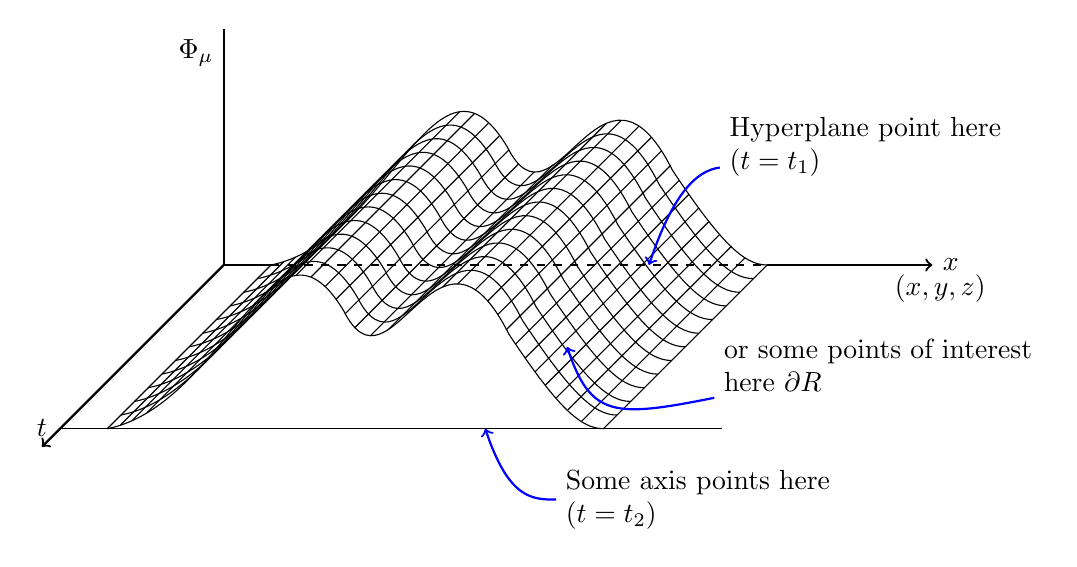
\begin{tikzpicture}[scale=3,block/.style={text width=11.2em}]
    % defining the coordinate axis
    \draw[thick] (0,0,0)--(0.2,0,0);
    \draw[dashed,thick] (0.2,0,0)--(2.3,0,0);
    \draw[->, thick] (2.3,0,0)--(3,0,0) node[right]{$x$};% x axis
    \draw[thick] (0,0,0)--(0,1,0) node[anchor=north east]{$\Phi_{\mu}$}; % field axis
    \draw[->,thick] (0,0,0)--(0,0,2) node[above]{$t$}; % t axis
    % draw the graphs
    \draw (0,0,1.8)--(2.8,0,1.8);
    \draw (0.2,0,1.8)--(0.2,0,0);
    \draw (2.3,0,1.8)--(2.3,0,0);
    \draw (0.2,0,0) .. controls (0.7,0.1,0) and (0.9,1,0) .. (1.2,0.5,0)
                    .. controls (1.4,0.1,0) and (1.6,1,0) .. (1.9,0.4,0)
                    .. controls (2.1,0.1,0) and (2.2,0.0,0) .. (2.3,0.0,0);
    \draw (0.2,0,0.15) .. controls (0.7,0.1,0.15) and (0.9,1,0.15) .. (1.2,0.5,0.15)
                    .. controls (1.4,0.1,0.15) and (1.6,1,0.15) .. (1.9,0.4,0.15)
                    .. controls (2.1,0.1,0.15) and (2.2,0.0,0.15) .. (2.3,0.0,0.15);
    \draw (0.2,0,0.3) .. controls (0.7,0.1,0.3) and (0.9,1,0.3) .. (1.2,0.5,0.3)
                    .. controls (1.4,0.1,0.3) and (1.6,1,0.3) .. (1.9,0.4,0.3)
                    .. controls (2.1,0.1,0.3) and (2.2,0.0,0.3) .. (2.3,0.0,0.3);
    \draw (0.2,0,0.45) .. controls (0.7,0.1,0.45) and (0.9,1,0.45) .. (1.2,0.5,0.45)
                    .. controls (1.4,0.1,0.45) and (1.6,1,0.45) .. (1.9,0.4,0.45)
                    .. controls (2.1,0.1,0.45) and (2.2,0.0,0.45) .. (2.3,0.0,0.45);
    \draw (0.2,0,0.6) .. controls (0.7,0.1,0.6) and (0.9,1,0.6) .. (1.2,0.5,0.6)
                    .. controls (1.4,0.1,0.6) and (1.6,1,0.6) .. (1.9,0.4,0.6)
                    .. controls (2.1,0.1,0.6) and (2.2,0.0,0.6) .. (2.3,0.0,0.6);
    \draw (0.2,0,0.75) .. controls (0.7,0.1,0.75) and (0.9,1,0.75) .. (1.2,0.5,0.75)
                    .. controls (1.4,0.1,0.75) and (1.6,1,0.75) .. (1.9,0.4,0.75)
                    .. controls (2.1,0.1,0.75) and (2.2,0.0,0.75) .. (2.3,0.0,0.75);
    \draw (0.2,0,0.9) .. controls (0.7,0.1,0.9) and (0.9,1,0.9) .. (1.2,0.5,0.9)
                    .. controls (1.4,0.1,0.9) and (1.6,1,0.9) .. (1.9,0.4,0.9)
                    .. controls (2.1,0.1,0.9) and (2.2,0.0,0.9) .. (2.3,0.0,0.9);
    \draw (0.2,0,1.05) .. controls (0.7,0.1,1.05) and (0.9,1,1.05) .. (1.2,0.5,1.05)
                    .. controls (1.4,0.1,1.05) and (1.6,1,1.05) .. (1.9,0.4,1.05)
                    .. controls (2.1,0.1,1.05) and (2.2,0.0,1.05) .. (2.3,0.0,1.05);
    \draw (0.2,0,1.20) .. controls (0.7,0.1,1.20) and (0.9,1,1.20) .. (1.2,0.5,1.20)
                    .. controls (1.4,0.1,1.20) and (1.6,1,1.20) .. (1.9,0.4,1.20)
                    .. controls (2.1,0.1,1.20) and (2.2,0.0,1.20) .. (2.3,0.0,1.20);
    \draw (0.2,0,1.35) .. controls (0.7,0.1,1.35) and (0.9,1,1.35) .. (1.2,0.5,1.35)
                    .. controls (1.4,0.1,1.35) and (1.6,1,1.35) .. (1.9,0.4,1.35)
                    .. controls (2.1,0.1,1.35) and (2.2,0.0,1.35) .. (2.3,0.0,1.35);
    \draw (0.2,0,1.5) .. controls (0.7,0.1,1.5) and (0.9,1,1.5) .. (1.2,0.5,1.5)
                    .. controls (1.4,0.1,1.5) and (1.6,1,1.5) .. (1.9,0.4,1.5)
                    .. controls (2.1,0.1,1.5) and (2.2,0.0,1.5) .. (2.3,0.0,1.5);
    \draw (0.2,0,1.65) .. controls (0.7,0.1,1.65) and (0.9,1,1.65) .. (1.2,0.5,1.65)
                    .. controls (1.4,0.1,1.65) and (1.6,1,1.65) .. (1.9,0.4,1.65)
                    .. controls (2.1,0.1,1.65) and (2.2,0.0,1.65) .. (2.3,0.0,1.65);
    \draw (0.2,0,1.8) .. controls (0.7,0.1,1.8) and (0.9,1,1.8) .. (1.2,0.5,1.8)
                    .. controls (1.4,0.1,1.8) and (1.6,1,1.8) .. (1.9,0.4,1.8)
                    .. controls (2.1,0.1,1.8) and (2.2,0.0,1.8) .. (2.3,0.0,1.8);

    \draw (0.25,0.01,1.785)--(0.25,0.01,-0.01);
    \draw (0.30,0.03,1.785)--(0.30,0.03,-0.01);
    \draw (0.35,0.05,1.755)--(0.35,0.05,0.7);
    \draw (0.43,0.13,0.56)--(0.43,0.13,0.17);
    \draw (0.48,0.13,0.45)--(0.48,0.13,-1.35);
    \draw (0.55,0.13,0.47)--(0.55,0.13,-1.33);
    \draw (0.65,0.13,0.57)--(0.65,0.13,-1.22);
    \draw (0.75,0.13,0.71)--(0.75,0.13,-1.08);
    \draw (0.85,0.13,0.87)--(0.85,0.13,-0.930);
    \draw (0.95,0.13,1.03)--(0.95,0.13,-0.775);
    \draw (1.05,0.13,1.115)--(1.05,0.13,-0.685);
    \draw (1.1,0.13,1.05)--(1.1,0.13,-0.765);
    \draw (1.15,0.13,0.58)--(1.15,0.13,-1.22);
    \draw (1.2,0.13,0.546)--(1.2,0.13,-1.25);
    \draw (1.3,0.13,0.616)--(1.3,0.13,-1.187);
    \draw (1.4,0.13,0.735)--(1.4,0.13,-1.065);
    \draw (1.5,0.13,0.88)--(1.5,0.13,-0.92);
    \draw (1.6,0.13,1.05)--(1.6,0.13,-0.76);
    \draw (1.7,0.13,1.21)--(1.7,0.13,-0.59);
    \draw (1.8,0.13,1.36)--(1.8,0.13,-0.44);
    \draw (1.9,0.13,1.51)--(1.9,0.13,-0.29);
    \draw (2.0,0.13,1.66)--(2.0,0.13,-0.14);
    \draw (2.1,0.13,1.8)--(2.1,0.13,0);
    \draw (2.15,0.08,1.8)--(2.15,0.08,0);
    \draw (2.196,0.02,1.77)--(2.196,0.02,-0.03);
% nodes: description of the regions and hypersurface
    \node[below right] at (2.8,0,0) {$\left(x,y,z\right)$};
    \path[block] (2.1,0.5,0) node[right] (x){Hyperplane point here ($t=t_{1}$)};
    \path[block] (2.1,-0.3,1.8) node[right] (y){Some axis points here ($t=t_{2}$)};
    \path[block] (2.5,0,1.1) node[right] (z){or some points of interest here $\partial R$};
    \draw[->,thick,blue] (x) .. controls (2.0,0.4,0) and (1.9,0.3,0) .. (1.8,0,0);
    \draw[->,thick,blue] (y) .. controls (2.0,-0.3,1.8) and (1.9,-0.3,1.8) .. (1.8,-0,1.8);
    \draw[->,thick,blue] (z) .. controls (2.0,-0.3,0.9) and (1.9,-0.3,0.9) .. (1.8,-0,0.9);
    
    \end{tikzpicture}
    \caption{Caption explaining significance of the image}
    \label{fig:my_label}
\end{figure}

\section{Mathematical Statements and Programs}

\begin{equation}
\frac{d\gamma}{dt} > 0,
\frac{d^2\alpha}{dt^2} > 0,
\forall t > 0.
\end{equation}

\end{sloppypar}